\chapter{Progettazione del Sistema}
\label{chap:systemdesign}
In questo capito si illustrerà il funzionamento attuale del sistema, analizzando le tecnologie che utilizza e accennando alle soluzioni pensate per ogni specifico problema. Inoltre si presenterà il modello di sviluppo dell'\emph{ingegneria del software} seguito.

\section{Reverse Enginering}
\newtheorem*{def:reverseengineering}{Definizione}
\begin{def:reverseengineering}
    La reingegnerizzazione è quel processo di esame, analisi e alterazione di un sistema software esistente, col fine di ricostruirlo in una nuova forma, e la successiva implementazione. \cite{chikofsky:reverseengineering} Nel processo di reingegnerizzazione è compresa anche la riprogettazione del software, mentre quando si parla di reverse engineering si fa riferimento alla sola analisi.
\end{def:reverseengineering}
Il reverse engineering del codice permette di invertire i processi di sviluppo e produzione di un software e quindi di ottenere uno sguardo prezioso dietro le quinte di un programma. Attraverso lo studio dettagliato del codice sorgente è possibile comprendere, riscrivere o ricostruire l’architettura di un programma, il suo funzionamento e le sue strutture interne. Apparentemente la reingegnerizzazione non dovrebbe essere fatta per modificare i requisiti funzionali del sistema. In realtà, spesso quando si applica questa tecnica ci si accorge, in fase di riprogettazione, che alcuni requisiti, dopo anni di sviluppo, non sono più validi e andrebbero tolti dal disegno, mentre altri, nuovi, andrebbero introdotti.

\subsection{I motivi}
La pandemia di quest'ultimo anno ha portato l'azione di refactoring su \emph{Zerocoda} ad essere a tutti gli effetti una necessità. Il distanziamento sociale è un bisogno per ogni tipo servizio offerto ad una clientela più o meno vasta, e tenere traccia dei clienti e del loro numero temporizzando gli accessi al servizio è senza alcun dubbio la soluzione migliore. Nello stato attuale, tuttavia, l'applicazione non rispetta i requisiti funzionali per essere rilasciata ad un pubblico di tipo \emph{enterprise}. Sono sempre di più le azienda che hanno richiesto l'inserimento dei loro servizi nell'applicazione. L'inserimento di nuovi servizi porterebbe all'aumento delle richieste da parte dei client, più richieste a più dati da elaborare, e più dati a un sovraccarico. L'applicazione non è pronta a uno scenario di questo tipo, pertanto urge un refactoring mirato all'introduzione di nuove tecnologie, che renda il software più scalabili, in prevenzione al nuovo numero di clienti sulla piattaforma.

Questo tuttavia rappresenta solo uno dei motivi, il principale, quello che ha portato l'azione di refactoring, dapprima solo ipotizzata da coloro che già lavoravano al sistema, a un inizio di progettazione. Normalmente le esigenze possono essere anche altre:

\begin{itemize}
    \item il team di sviluppo è cambiato e sono subentrati altri programmatori che non hanno conoscenze in merito al sistema;
    \item la documentazione è assente del tutto o, se presente, dopo anni di sviluppo e modifiche non è stata aggiornata e risulta obsoleta;
    \item  l'introduzione di piccoli cambiamenti risulta complessa e costosa da affrontare in termini di tempo e risorse;
    \item il software è spesso soggetto a continue correzioni di bug, indice che la struttura è precaria e mal progettata;
    \item numerose correzioni sono state apportare e si è verificato il fenomeno ``architectural drift'' (deriva architetturale), cioè il sistema si è spostato molto dal disegno originale che non è più chiaro
    \item i metodi e gli strumenti di sviluppo originali sono ormai superati ed è difficile trovare programmatori con queste conoscenze.
\end{itemize}

%%%%%%%%%%%%%%%%%%%%%%%%%%%%%%%%%%%%%%%%%%%%%%%%%%%%%%%%%%%%%%%%%%%%%%%%%
\section{Modello di Sviluppo}
Come \textit{metodologia di sviluppo} si è scelto di adottarne una di tipo \textbf{agile}. Secondo questo \emph{principio teorico}, il punto di partenza è costituito dalla specifica dei requisiti, mentre lo sviluppo vero e proprio del software avviene solo in seguito.

\subsection{Waterfall Model}
Il modello a cascata è un \textbf{ciclo di vita lineare}, che suddivide il processo di sviluppo in fasi di progetto consecutive. A differenza dei modelli iterativi, \textit{ogni fase viene eseguita solo una volta}. Con questo modello il progetto viene organizzato in una sequenza di fasi, ciascuna delle quali produce un output che costituisce l’input per la fase successiva.

\subsubsection{Origini}
Lo sviluppo del modello viene attribuito allo scienziato informatico Winston W. Royce, che tuttavia, non è stato il suo vero inventore. Al contrario, il suo articolo pubblicato nel 1970 “Managing the Development of Large Software Systems” \cite{royce:softwaredevelopment} conteneva una critica aperta nei confronti dei cicli di vita lineari. Come alternativa, presentava un modello iterativo-incrementale, in cui ogni fase attinge a quella precedente e ne verifica i risultati. 

\paragraph{Il modello di Royce} è cosituito da sette fasi eseguite in diversi passaggi (iterazioni):

\begin{enumerate}
    \item Requisiti di sistema
    \item Requisiti di software
    \item Analisi
    \item Progettazione
    \item Implementazione
    \item Test
    \item Esecuzione e Manutenzione
\end{enumerate}
Il modello a cascata si ispira alle fasi definite da Royce, ma prevede solo un’iterazione.

\subsubsection{Funzionamento}
Nella pratica vengono utilizzate diverse versioni del modello a cascata. Attualmente sono in uso modelli che suddividono i processi di sviluppo in cinque fasi. Le fasi 1, 2 e 3, definite da Royce, sono riunite in un’unica fase di progetto, chiamata analisi dei requisiti.
\begin{enumerate}
    \item Analisi: pianificazione, analisi e specificazione dei requisiti
    \item Progettazione: progettazione e specificazione del sistema
    \item Implementazione: programmazione e test di modulo
    \item Test: integrazione di sistema, test di sistema e test di integrazione
    \item Esecuzione: rilascio, manutenzione, miglioramento
\end{enumerate}
\begin{figure}[H]
    \centering
    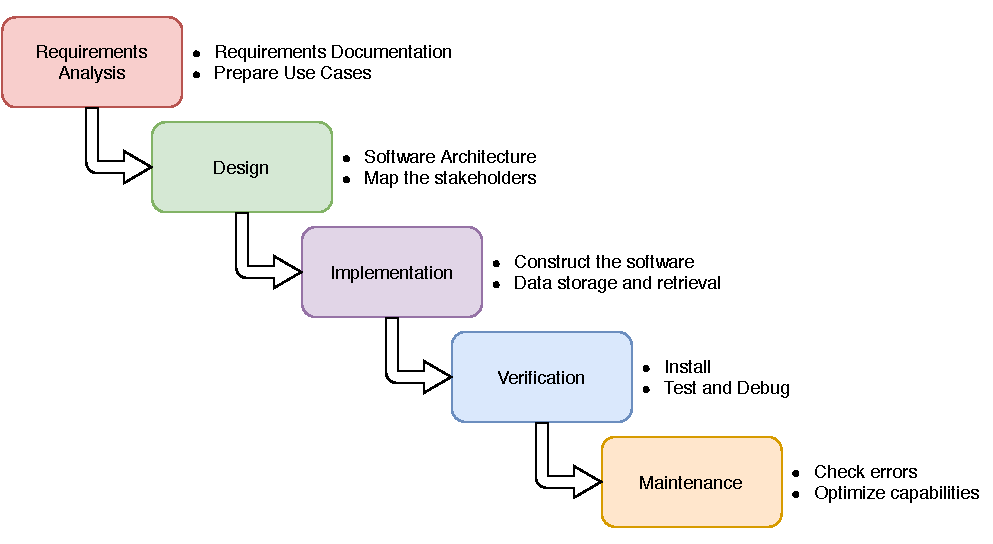
\includegraphics[width=0.94\textwidth]{images/02_1_waterfall_model.pdf}
    \caption{Fasi del Modello a Cascata}
    \label{fig:waterfallmodel}
\end{figure}

Il modello da noi utilizzato rappresenta un'\textit{estensione del modello a cascata}, in quanto l'eseguire ogni fase una sola volta comporta un grande vincolo. Ad ogni fase infatti si confrontano e verificano i risultati ottenuti con quelli della fase precedente. Partendo da un'analisi delle esigenze richieste dall'applicazione, dai suoi limiti e dalle necessità dei clienti, si è poi passati all'individuazione di una strada per lo sviluppo.

%%%%%%%%%%%%%%%%%%%%%%%%%%%%%%%%%%%%%%%%%%%%%%%%%%%%%%%%%%%%%%%%%%%%%%%%%
\section{Funzionamento dell'Applicazione}

\subsection{Scenario}
Lo scopo di quest'applicazione è quello di \textit{velocizzare l'accesso i servizi}. Senza questo \textit{primo requisito}, l'applicazione non troverebbe posto nel mondo enterprise. Per questo motivo, l'interfaccia utente risulta semplice, e comprende poche funzionalità. 
\paragraph{L'utente} per accedere ai servizi deve registrarsi al sistema fornendo i propri dati personali (che potranno essere modificati in qualsiasi momento), scegliendo un'email e una password per le future autenticazioni. Una volta registrato, può cercare una struttura tra quelle presenti e scegliere un servizio che questa eroga. 
\paragraph{I servizi} possono essere diversi: analisi, esami, visite mediche, qualsiasi servizio che preveda un'attesa del cliente potrebbe essere inserito da una struttura sanitaria. Selezionando un servizio, all'utente viene mostrato il relativo calendario di disponibilità, i termini di giorni e fasce orarie. 
\paragraph{La prenotazione} avviene una volta selezionato un orario (corrispondente a uno \emph{slot}) e confermata l'intenzione di volerlo riservare. Prima di confermare, l'utente registrato può scegliere di inserire i dati (almeno uno tra nome e cognome, email o numero di telefono) di un altro utente, anche non iscritto al sistema, per cui prenotare il servizio. Scegliendo questa il destinatario sarà informato mediante delle notifiche sui futuri eventi relativi allo stato della sua prenotazione. A questo punto all'utente viene fornito un ``biglietto virtuale''.
\paragraph{Il biglietto} consiste in una numerazione. Questa numerazione corrisponde al numero che verrà chiamato allo sportello (si pensi ad un biglietto virtuale staccato al momento della prenotazione). Ciascun servizio è identificato da una lettera dell’alfabeto (A, B, C, \dots) mentre ciascun numero identifica il cliente in coda (1, 2, 3, \dots). In questo modo la numerazione B12, ad esempio, fa riferimento al cliente numero 12 di un servizio, C13 ad un altro cliente di un altro servizio. L’idea è che chi ha prenotato acceda alla struttura nel momento esatto in cui viene erogato il servizio, evitando coda e assembramenti.
\paragraph{La struttura}, così come l’utente, deve avere informazione di questo biglietto virtuale e questo avviene attraverso un \textsl{software} installato nelle strutture che prende il nome di \textbf{mru}.
\paragraph{L'MRU} è un software che disponde di un'interfaccia web per gli operatori e per i totem che vengono utilizzati. Tutte le notti l'MRU interroga Zerocoda richiedendo le prenotazioni per la giornata odierna. Se ci sono le scarica, in questo modo anche gli operatori hanno informazione delle prenotazioni.

\subsection{Use Case Diagram}
\begin{figure}[H]
    \centering
    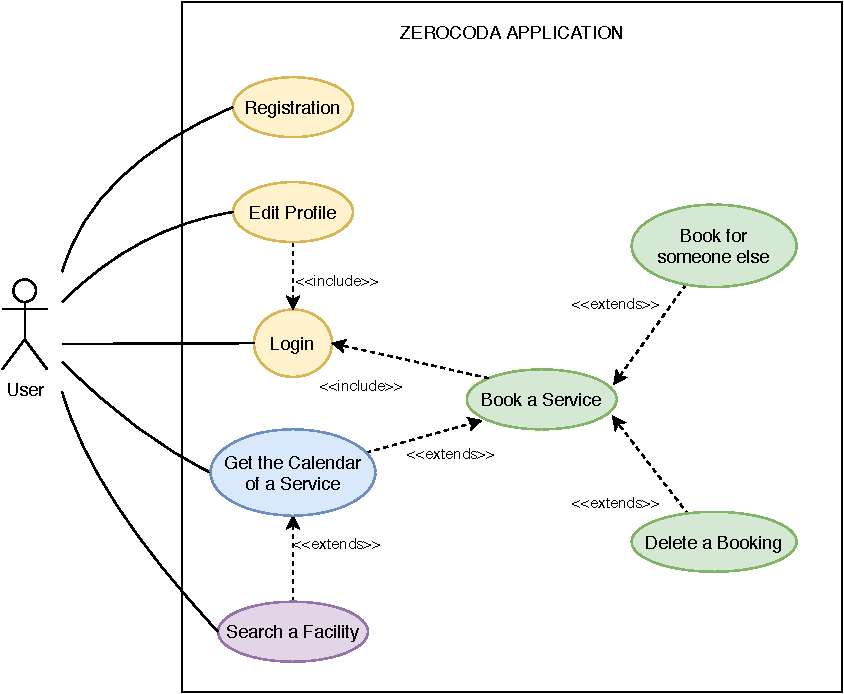
\includegraphics[width=0.94\textwidth]{images/02_2_zerocoda_usecase.pdf}
    \caption{Zerocoda Use Case Diagram}
    \label{fig:zerocodausecase}
\end{figure}
I diversi colori utilizzati rappresentano la \textit{divisione in servizi} scelta per la fase di implementazione delle REST Api.

%%%%%%%%%%%%%%%%%%%%%%%%%%%%%%%%%%%%%%%%%%%%%%%%%%%%%%%%%%%%%%%%%%%%%%%%%
\section{Analisi dell'Applicazione}
\subsection{I diversi Enti di Zerocoda}
Sull'applicazione Zerocoda è possibile prenotare i servizi erogati da diversi enti. Alcuni di questi, tuttavia, non sono presenti sul sito. Ci sono strutture sanitarie che non vogliono che i loro utenti accedano a un sito generalista come \textsf{Zerocoda.it}. Questi vogliono che il loro sito funga da ``vetrina'', che l'utente riconosca la struttura presso cui prenota attraverso elementi come il logo, il nome, ecc\dots L'utilizzo del \textbf{virtual hosting} risponde a questa esigenza. In fase di accesso il servizio compare come se fosse erogato dell’ente privato. Questi \textit{siti premium} consistono in realtà in un sito statico (come lo stesso Zerocoda), ma con una configurazione dedicata, che una volta ricevuta dal browser cambia il \textsf{look and feel}.

\paragraph{É possibile offrire una  personalizzazione maggiore} ai siti che la richiedono. La richiesta può essere quella dell'utilizzo di colori particolari per gli elementi della pagina: quali pulsanti, form, colori del background.

\paragraph{La configurazione} consiste in un file JSON contenente tutte le informazioni del sito. Oltre alle informazioni relative al nome, indirizzo, descrizione, contiene anche stringhe di testo già formattate in HTML, da inserire all'interno della pagina in appositi spazi. Può contenere anche informazioni riguardanti lo stile (CSS) della pagina. La configurazione viene caricata per ultima, dopo che i componenti statici sono stati renderizzati. Viene inviata al frontend attraverso uno script JavaScript.

\paragraph{In numeri}, i clienti (enti sanitari) per Zerocoda sono 45. Il numero comprende sia gli enti presenti su Zerocoda, sia coloro che hanno richiesto una personalizzazione su un proprio portale. Il sistema, in totale vanta i seguenti numeri:
\begin{itemize}
    \item 1 Zerocoda
    \item 17 siti con configurazione personalizzata
    \item 500.000 utenti registrati
    \item 298 impianti di MRU registrati
\end{itemize}


\subsection{Multitenancy e Virtual Hosting}
La particolarità del sistema è quella di essere \textbf{multitenant}. Con un solo servizio è possibile offfrire esperienze isolate agli utenti: una diversa esperienza sulla base della loro organizzazione. In questo modo, se un nuovo ente richiedesse che tutti i suoi dati fossero salvati su un nuovo database, si potrebbe installare un nuovo ambiente separato apposito. In alcuni casi è possibile anche chiedere metodi di registrazione o accesso al sistema ad-hoc, evitando il sistema standard basato su email e password. Così facendo, il sistema si limiterebbe ad esporre un'API in aggiunta all'applicazione condivisa da tutti, che gestisce la richiesta di autenticazione personalizzata sulle necessità dell'ente richiedente.
\begin{figure}[H]
    \centering
    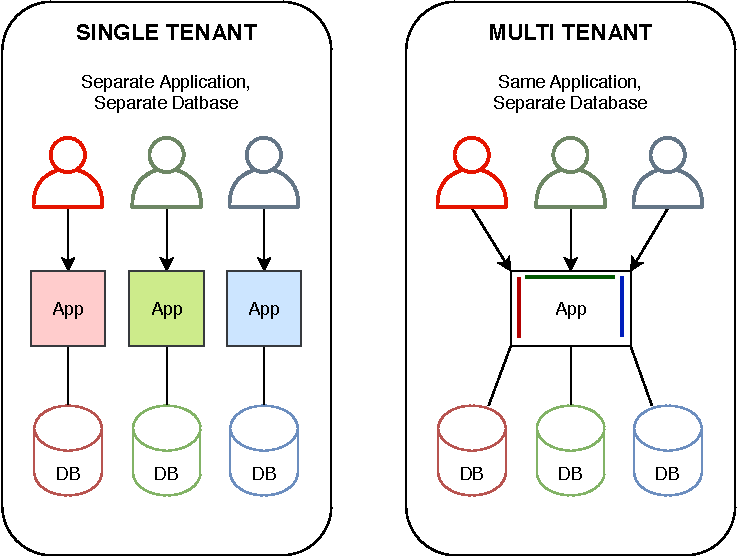
\includegraphics[width=0.94\textwidth]{images/02_3_multitenancy.pdf}
    \caption{Single Tenant vs. Multi Tenant}
    \label{fig:multitenancy}
\end{figure}

\subsection{Backend Overview}
Ad oggi non è attualmente presente un elemento definibile come \emph{layer di API} nell’applicazione. Il sistema è composto da un unico monolite che tra le tante mansioni che ha espone anche le `API'. Nello stesso sistema viene effettuato ogni genere di controllo per quanto rigurarda l'autenticazione e i parametri passati nelle richieste. Il backend è interamente scritto in PHP e si appoggia ad un database MySQL. Nonostante con gli ultimi aggiornamenti PHP offra la possibilità di programmare a oggetti, questo non è il caso del sistema preso in analisi. Per la creazione di dati che in altri linguaggi sarebbero rappresentabili attraverso oggetti, il backend utilizza un sistema di liste con elementi di tipo chiave-valore.

\subsection{Chiamate delle API}
Le chiamate dal frontend alle API intercettano il click sul documento, andando a cercare il componente su cui è stata registrata l'interazione. Tutte le richieste inviate al backend sono richieste GET HTTP. Quindi, passando un qualsiasi parametro o effettuanto operazioni di aggiunta o modifica di dati, i parametri vengono aggiunti all'url, e mostrati in chiaro. Questo scelta è stata adottata anche per i metodi di registrazione e autenticazione, i più delicati dal punto di vita della sicurezza. Con la sintassi \textsl{\$\_GET} in PHP si fa riferimento a una variabile globale che contiene i parametri in GET della richiesta HTTP.
\begin{figure}[H]
\begin{alltt}
    \centering
    http://domain.it/index.php/api/v1/login?
    \centering
    _apikey=1&
    &email=prova123%40gmail.com&
    password=Prova123!
\end{alltt}
\caption{Richiesta GET in HTTP}
\end{figure}

(tipicamente i paraemtri dell'URL). Questa variabile tuttavia può anche contenere altri dati che è possibile aggiungere. L'ID ad esempio è parte di quei dati aggiunti dal framework che non si troverà nella richiesta in INPUT.

%%%%%%%%%%%%%%%%%%%%%%%%%%%%%%%%%%%%%%%%%%%%%%%%%%%%%%%%%%%%%%%%%%%%%%%%%

%%%%%%%%%%%%%%%%%%%%%%%%%%%%%%%%%%%%%%%%%%%%%%%%%%%%%%%%%%%%%%%%%%%%%%%%%

%%%%%%%%%%%%%%%%%%%%%%%%%%%%%%%%%%%%%%%%%%%%%%%%%%%%%%%%%%%%%%%%%%%%%%%%%

%%%%%%%%%%%%%%%%%%%%%%%%%%%%%%%%%%%%%%%%%%%%%%%%%%%%%%%%%%%%%%%%%%%%%%%%%

%%%%%%%%%%%%%%%%%%%%%%%%%%%%%%%%%%%%%%%%%%%%%%%%%%%%%%%%%%%%%%%%%%%%%%%%%